% Copyright (C) 2011 Thomas L. Kula
% All Rights Reserved
%
% See the file LICENSE for license terms.
\documentclass[12pt]{article}
\usepackage{graphicx}
\usepackage{rotating}
\usepackage{fix-cm}
\usepackage{multirow}
\setlength{\paperwidth}{5.5in}
\setlength{\paperheight}{8.5in}
\setlength{\textheight}{7.45in}
\setlength{\topmargin}{-1.0in}
\setlength{\oddsidemargin}{-0.5in}
\setlength{\evensidemargin}{-0.5in}
\setlength{\textwidth}{4.0in}
\setlength{\parindent}{0in}
\setlength{\parskip}{3mm}
\usepackage[print]{booklet} \nofiles
\source{\magstep0}{5.5in}{8.5in}
\target{\magstep0}{11in}{8.5in}
\setpdftargetpages
\pagestyle{empty}
\begin{document}


\begin{center}
{\fontsize{36}{48}\selectfont \textsc{Haiku a Day }}
\end{center}

\vspace*{3.5cm}

{\fontsize{20}{40}\selectfont 

Why do I have this?

I never unpacked that box.

Get rid of it all.


}

\vspace*{5.0cm}
\begin{center}
{\large{Issue 75: September 2011}} \\[5mm]
{\fontsize{8}{8}\selectfont  \textsc{ St. Joshua Norton Press }} \\[1mm]
{\fontsize{6}{6}\selectfont Mathom House in Midtown \textbar The People's Republic of Ames }
\end{center}


\newpage

I've donated, recycled or disposed of probably 80\% of everything I own.
It's a liberating experience.

New address coming soon --- stay tuned for the next issue, coming
to you from New York City.

--- Thomas

http://kula.tproa.net/had/ \\
kula@tproa.net

Download this and previous HADs at the website, so you can
print out your own (DIY, yeah!) or if you want me to send
you one, send me your address, and maybe a stamp if you
are feeling nice. Or send me something you've made ---
trades always appreciated, postcards are nice too.

\vfill

1 Sept 2011

One, single digit \\
Keeps multipliers the same \\
To build more, just add

2 Sept 2011

Two, doubling power \\
Binary's simple basis \\
Only even prime

\newpage

3 Sept 2011

Times for luck, at bat \\
Three legs on a stool keeps you \\
From falling over

4 Sept 2011

Corners of the earth \\
From there four winds blowing forth \\
Swaying the grasses

5 Sept 2011

This song in my head \\
Has been going all morning \\
Will it ever stop?

6 Sept 2011

The whirr of a fan \\
Complimenting a soft breeze \\
Putting me to sleep

7 Sept 2011

The smell of chalk dust \\
Bringing back fond memories \\
Daydreaming of school

8 Sept 2011

Office vent like jet \\
A constant background droning \\
Scares me when it stops

9 Sept 2011

Rustle above me \\
Birds are in the eaves again \\
Twitter merrily

\newpage

10 Sept 2011

Toucan Sam waves hi \\
Smiling on my coffee mug \\
Is this brew fruity?

11 Sept 2011

This code is hacky \\
Somehow, though, I made it work \\
Surprised me to hell

12 September 2011

New job accepted \\
I go to New York City \\
Now I have to move

13 September 2011

Lined up in a row \\
Quarters make the washer go \\
Making my clothes clean

14 September 2011

Thank you, scratchy throat \\
You make me sound like a frog \\
Amputate, I say

15 September 2011

Still in my cupboard \\
Aluminum foil roll \\
From the Ames HyVee

16 September 2011

Flickering light bulb \\
How you make me hate this place \\
Pick on or off, please


\newpage

17 September 2011

Think apple cider \\
Remember cider doughnuts \\
Sigh a happy sigh

18 September 2011

Boxes still unpacked \\
From the last move, throw away \\
I don't need that stuff

19 September 2011

Harder than I thought: \\
Getting rid of a new car \\
Must go: Ohio

20 September 2011

Thousands of details \\
Overwhelm a puny mind \\
Checklist sanity

21 September 2011

Online newspapers \\
Have but one cardinal rule: \\
Never read comments

22 September 2011

Flashing lights go by \\
And the siren draws like I'm \\
Still a little kid

23 September 2011

Staring at the sky \\
Don't know what I'm looking for \\
Perhaps it's nothing


\newpage

24 September 2011

Staring at fire \\
The glow of embers soothes me \\
Simple happiness

25 September 2011

Connections pay off \\
A cousin in NYC \\
Gives apartment leads

26 September 2011

The thought of dishes \\
Filling with a sense of dread \\
Do them already

27 September 2011

Here I come, New York \\
I'm going to find a place \\
Get out of my way

28 September 2011

Hours of walking \\
Trying to find a new home \\
Up and down we go

29 September 2011

Large sums of money \\
If you want an apartment \\
Make my account pale

30 September 2011

An apartment found \\
I breathe a sigh of relief \\
And sleep more soundly


\newpage

\begin{center}
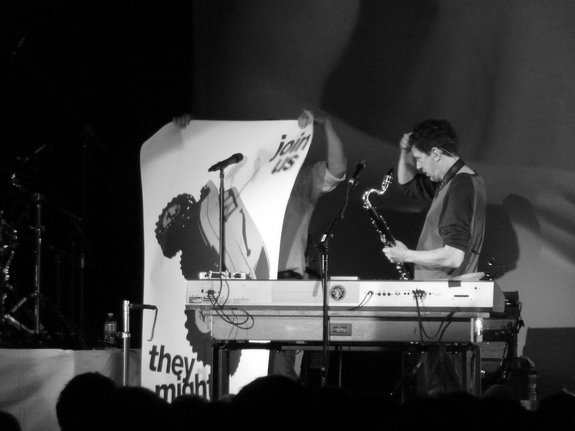
\includegraphics{tmbg-small.png}

They Might Be Giants, Majestic Theater, Detroit --- 17 September 2011 \\
{\tt kula.tproa.net/photos/2011/20110917-tmbg }
\end{center}


\newpage

\thispagestyle{empty}
\vspace*{12cm}
\begin{sideways}
\Large{St. Joshua Norton Press}
\end{sideways}
\begin{sideways}
\Large{PO Box 980461}
\end{sideways}
\begin{sideways}
\Large{Ypsilanti MI 48198}
\end{sideways}


\end{document}


